\documentclass[tikz,border=2pt]{standalone}
\renewcommand{\familydefault}{\sfdefault}
\usetikzlibrary{arrows.meta,calc,positioning}
\tikzset{every picture/.style={line width=1pt, >=Stealth},
         hl/.style={fill=black, fill opacity=0.12, text opacity=1}}
\begin{document}
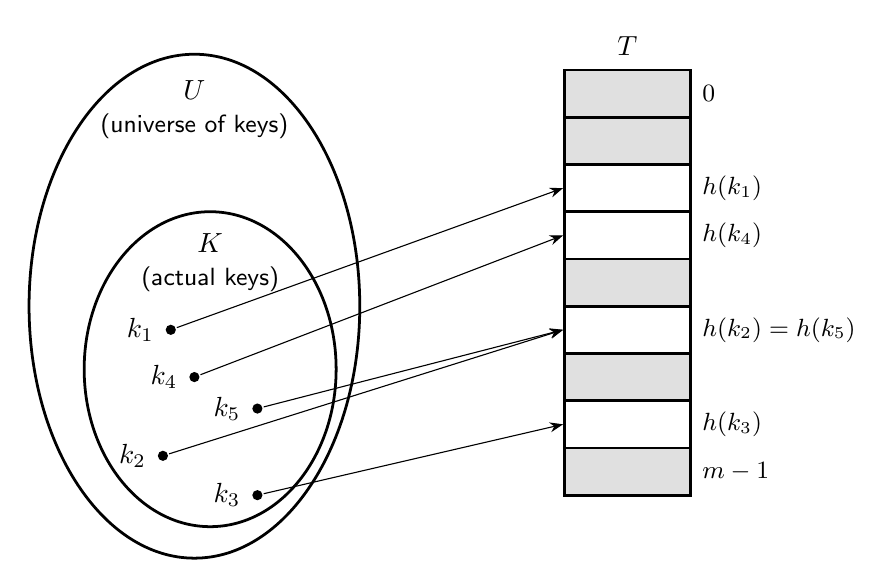
\begin{tikzpicture}[slot/.style={draw, minimum width=1.6cm, minimum height=0.6cm}, key/.style={circle, fill, inner sep=1.3pt}]
  % Universe U of possible keys, containing the keys K actually stored.
  \draw (0, 0) ellipse (2.1cm and 3.2cm);
  \node[align=center] at (0, 2.5) {$U$ \\ \small(universe of keys)};
  \draw (0.2, -0.8) ellipse (1.6cm and 2cm);
  \node[align=center] at (0.2, 0.55) {$K$ \\ \small(actual keys)};

  % Table T with m slots; shaded slots are empty.
  \node at (5.5, 3.3) {$T$};
  \foreach \i in {0, ..., 8} \node[slot] (t\i) at (5.5, 2.7 - 0.6*\i) {};
  \foreach \i in {0, 1, 4, 6, 8} \node[slot, hl] at (t\i) {};
  \node[right, font=\small] at (t0.east) {$0$};
  \node[right, font=\small] at (t8.east) {$m - 1$};

  \foreach \k/\x/\y/\slot/\label in {1/-0.3/-0.3/2/{h(k_1)}, 4/0/-0.9/3/{h(k_4)},
      5/0.8/-1.3/5/{h(k_2) = h(k_5)}, 2/-0.4/-1.9/5/{}, 3/0.8/-2.4/7/{h(k_3)}} {
    \node[key, label=left:$k_\k$] (k\k) at (\x, \y) {};
    \draw[->, thin] (k\k) -- (t\slot.west);
    \node[right, font=\small] at (t\slot.east) {$\label$};
  }
\end{tikzpicture}
\end{document}
